
In contrast to the discrete two-point distribution, we also analyzed
the relative overrepresentation of bidirectional connections in a
network with continuously distributed connection probabilities. The
gamma distribution $\Gamma(\alpha, \beta)$ with probability density
function
\begin{align}
    f_{\alpha,\beta}(x) = \begin{cases} 
\frac{1}{\beta^{\alpha}\Gamma(\alpha)}\, x^{\alpha-1}\,e^{-x/\beta} & x \geq 0 \\
0 & \text{otherwise},
\end{cases}
\end{align}
allows the variation the variance $\Var(X)= \alpha \beta^2 $ of a
gamma distributed random variable $X \sim \Gamma(\alpha, \beta)$ while
keeping its mean $\E(X) = \alpha \beta $ constant \cite{Hogg1978}.
%\cc{pages 103-105}
The exponential distribution emerges as a special case of the gamma
distribution ($\alpha =1$).

Here we consider a slight modification to the traditional gamma
distribution in the form of a truncated version. Let $\alpha, \beta >
0$. A random variable $X$ follows the truncated gamma distribution
$\Gamma^T(\alpha, \beta)$ if it has the probability density function
%
\begin{align}
  f_{\alpha,\beta}^T(x) = \begin{cases} K_{\alpha, \beta}\,
\frac{1}{\beta^{\alpha}\Gamma(\alpha)}\, x^{\alpha-1}\,e^{-x/\beta} & 0 \leq x \leq 1 \\
0 & \text{otherwise}.
\end{cases}
\end{align}
%
The factor $K_{\alpha,\beta}$ is needed due to the truncation of the
probability density function for $x>0$ to ensure that
\begin{align}
  \int f_{\alpha,\beta}^T(x) \,dx = 1 \label{eq:gd1},
\end{align}
and $K_{\alpha,\beta}$ is determined as the inverse of the cumulative
probability $x \leq 1$ of the untruncated gamma distribution,
\begin{align}
  K_{\alpha,\beta} = \left(\int_0^{1} f_{\alpha,\beta}(x) \, dx \right)^{-1}.
\end{align}
With this the equality~\eqref{eq:gd1} clearly holds. Consider then the
above network model in which the connection probabilities $P_{ij}$ are
$\Gamma^T(\alpha, \beta)$ distributed. We computed the relative
overrepresentation $\varrho$ from $\mu = E(P_{ij})$ and $E(P_{ij}^2)$
from
\begin{align}
  \mu = \E(P_{ij}) &= \int_0^1 x f_{\alpha,\beta}^T(x)\, dx,\\
        \E(P_{ij}^2) &= \int_0^1 x^2 f_{\alpha,\beta}^T(x)\, dx.
\end{align}
Pairings of the shape parameter $\alpha$ and the scale parameter
$\beta$ were chosen such that the overall connection probability
reflects connectivity statistics in local cortical networks, $\mu =
1$. Probability density functions and resulting relative
overrepresentation of reciprocal connections $\varrho$ for four
representative $\alpha,\beta$ pairs are shown in
Figure~\ref{fig:gd}A. In the sparse networks we modeled ($\mu = 0.1$),
we find that the truncated gamma distribution can be well approximated
by the \cc{non truncated version}, $K_{\alpha, \beta} \approx 1$.

Assuming the $P_{ij}$ to be standard gamma distributed, 

We note the following results for the overall connection probability
$\mu$,
%
\begin{align}
 \mu = \E(P_{ij}) = \alpha \beta, \label{eq:gd3}.
\end{align}
Figure~\ref{fig:gd}B shows that the relationship $\beta =
\frac{\mu}{\alpha}$ holds well for $\mu = 0.1$ and $\alpha > 1$. The
expected occurrence of bidirectional connections is
\begin{align}
  \E(P_{ij}^2) = \alpha^2 \beta^2 + \alpha \beta^2,
\end{align}
%
and the overrepresentation is then
\begin{align}
  \varrho & = \frac{\E(P_{ij}^2)}{\E(P_{ij})^2} =% \frac{\alpha^2 \beta^2}{\alpha^2 \beta^2} + \frac{\alpha \beta^2}{\alpha^2 \beta^2} =
 1 + \frac{1}{\alpha}.
\end{align}

We see that for sparse networks, this approximation holds in for $\alpha \geq 1$ (Figure~\ref{fig:gd}\textbf{C}).

\begin{figure}[h!]
\centering
%\includegraphics[width=0.703\textwidth]{../lab/gamma_distribution/gamma_figure.png}
%\includegraphics[width=0.287\textwidth]{../lab/gamma_distribution/gamma_figure_logscale.png}
\includegraphics[width=\textwidth]{../figures/gamma_distribution/gamma_figure.pdf}
\caption{\textbf{A} Probability density functions of the truncated
  gamma distribution for different shape parameters $\alpha$ and the
  induced relative overrepresentation of bidirectional connections
  $\varrho$ in a network with such distributed connection
  probabilities $P_{ij}$. For given $\alpha$ the parameter $\beta$ was
  estimated numerically to yield $\mu \approx 0.1$ in all
  distributions shown.}
\label{fig:gd}
\end{figure}

In Figure~\ref{fig:gd} probability density functions for multiple
parameter sets $(\alpha, \beta)$ are shown. The rate parameter $\beta$
is determined by the given $\alpha$ and $\mu = 0.1$ through the
relation in \eqref{eq:gd3}. [Comment: I'm not sure it's worth deriving
  an expression for $\beta$. A good approximation is $\beta =
  \frac{\mu}{\alpha}$, ($K_{\alpha,\beta} = 1$). I just need to make
  it clear what I'm doing.]

The narrower the probability density around the mean $\mu = 0.1$ the
smaller is the expected overrepresentation of bidirectional
connections $\varrho$ in the network. To achieve a high $\varrho$ many
pairs with a high connection probability are needed. The dashed line
in Figure~\ref{fig:gd} marks the probability density function of the
probability distribution of connection probabilities $P_{ij}$ that
induce an overrepresentation of reciprocal pairs of $\varrho = 4$ as
found by \textcite{Song2005} leading to a highly skewed distribution
with a long tail. The relevance of such a distribution for cortical
networks however is debatable, as most connections are with a high
certainty not established seemingly wasting the network's potential
for different possible configurations.


Notably, to achieve an overrepresentation of $\varrho = 4$ as found by
\textcite{Song2005} most of the pairs in the network are almost
certainly unconnected .


%References: \href{http://herbsusmann.com/distributions/gamma-distribution-variance-proof.html}{Proof $\E(X^2)$}, 

